\documentclass{article}

\usepackage{graphicx}
\usepackage{tikz}
\usepackage{tikzsymbols}
\usetikzlibrary{calc,patterns,shapes.geometric}
\pagestyle{empty}
\usepackage[margin=0pt]{geometry}
\geometry{papersize={14in,12in}}

\def\centerarc[#1](#2)(#3:#4:#5){\draw[#1] ($(#2)+({#5*cos(#3)},{#5*sin(#3)})$) arc (#3:#4:#5);}

\begin{document}
	\begin{figure}
		\centering
		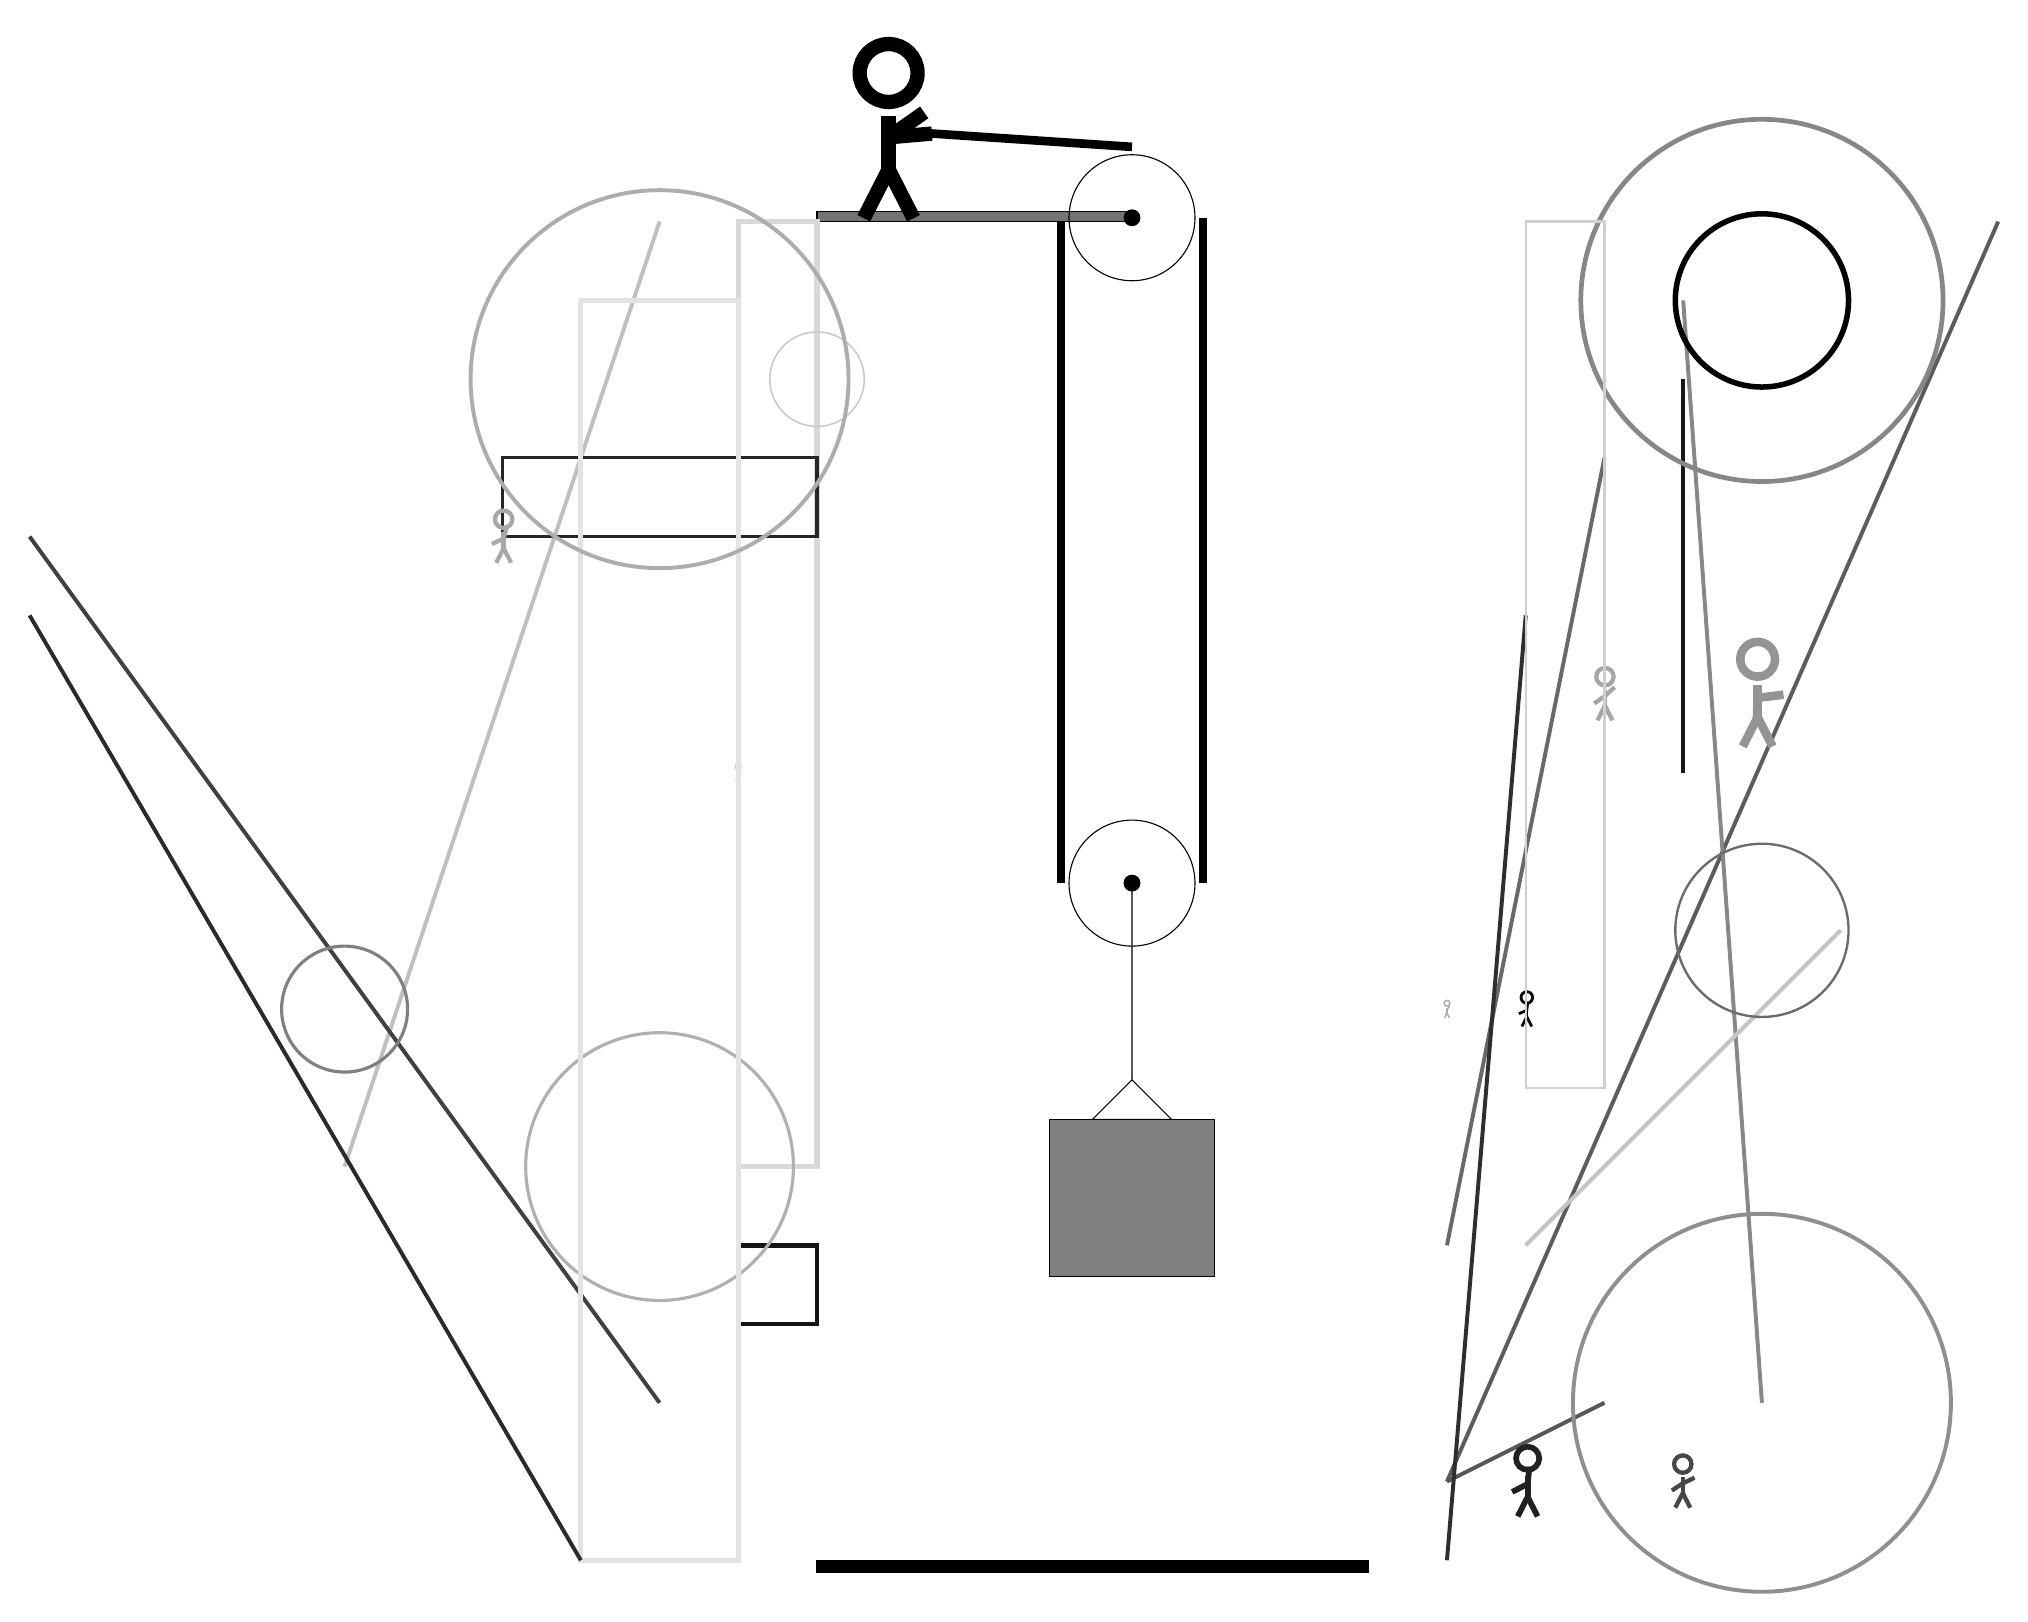
\begin{tikzpicture}
			%%%%% START %%%%%
			
			\draw[fill=black!55] (-2, 14) rectangle (2, 14.125);
			
			\node[line width=0.5mm, color=black!96] at (7, 4) {\Strichmaxerl[2][23][84]};
			
			\draw[line width=0.5mm, color=black!64](6, -2) -- (13, 14);
			\draw[line width=0.5mm, color=black!47](10, -1) -- (9, 13);
			\draw[line width=0.5mm, color=black!25](-4, 14) -- (-8, 2);
			
			\draw[line width=0.7mm, color=black!15] (-2, 14) rectangle (-3, 2);
			\draw[line width=0.6mm, color=black!92] (-2, 1) rectangle (-3, 0);
			\draw[line width=0.5mm, color=black!23](7, 1) -- (11, 5);
			
			\draw[line width=0.4mm, color=black!85] (-2, 10) rectangle (-6, 11);
			\node[line width=0.7mm, color=black!20] at (-3, 7) {\Strichmaxerl[1][88][43]};
			\node[line width=0.6mm, color=black!34] at (-6, 10) {\Strichmaxerl[3][25][74]};
			\draw [line width=0.2mm, color=black!21](-2, 12) circle (0.6);
			\draw[line width=0.5mm, color=black!75](-4, -1) -- (-12, 10);
			\node[line width=0.4mm, color=black!35] at (8, 8) {\Strichmaxerl[3][35][42]};
			\draw [line width=0.7mm, color=black!99](10, 13) circle (1.1);
			\draw [line width=0.4mm, color=black!31](-4, 2) circle (1.7);
			\draw [line width=0.4mm, color=black!50](-8, 4) circle (0.8);
			
			\draw[line width=0.5mm, color=black!66](8, -1) -- (6, -2);
			
			\draw[line width=0.6mm, color=black!11] (-3, 13) rectangle (-5, -3);
			\draw [line width=0.6mm, color=black!36](10, 6) circle (0.0);
			
			\draw[line width=0.5mm, color=black!91](9, 12) -- (9, 7);
			\draw[line width=0.5mm, color=black!83](-5, -3) -- (-12, 9);
			
			\draw [line width=0.5mm, color=black!32](-4, 12) circle (2.4);
			
			\draw[line width=0.5mm, color=black!59](6, 1) -- (8, 11);
			\node[line width=0.7mm, color=black!42] at (10, 8) {\Strichmaxerl[6][88][7]};
			\draw[line width=0.5mm, color=black!75](5, 2) -- (5, 2);
			\draw [line width=0.3mm, color=black!58](10, 5) circle (1.1);
			\node[line width=0.5mm, color=black!87] at (7, -2) {\Strichmaxerl[4][27][84]};
			\draw[line width=0.5mm, color=black!82](6, -3) -- (7, 9);
			\node[line width=0.3mm, color=black!72] at (9, -2) {\Strichmaxerl[3][33][26]};
			\node[line width=0.4mm, color=black!33] at (6, 4) {\Strichmaxerl[1][82][54]};
			\draw [line width=0.6mm, color=black!47](10, 13) circle (2.3);
			
			\draw[line width=0.3mm, color=black!19] (7, 3) rectangle (8, 14);
			\draw [line width=0.5mm, color=black!44](10, -1) circle (2.4);
			
			
			\draw (2, 5.6) circle (0.8);
			\draw[fill=black] (2, 5.6) circle (0.1);
			
			\draw (2, 14.05) circle (0.8);
			\draw[fill=black] (2, 14.05) circle (0.1);
			
			\draw (2, 5.6) -- (2, 3.1) -- (1.5, 2.6) -- (2.5, 2.6) -- (2, 3.1);
			\draw[fill=black!50] (0.95, 2.6) rectangle (3.05, 0.6);
			
			\draw[line width=1.1mm] (1.1, 14) -- (1.1, 5.6);
			\centerarc[line width=1.1mm](2, 5.6)(180:360:0.9);
			\draw[line width=1.1mm](2.9, 5.6) -- (2.9, 14.05);
			\centerarc[line width=1.1mm](2, 14.05)(0:90:0.9);
			\draw[line width=1.1mm](2, 14.95) -- (-1, 15.15);
			
			\node at (-1, 15.15) {\Strichmaxerl[10][-175][35]};
			
			\draw[fill=black] (-2, -3) rectangle (5, -3.15);
			
			%%%%% END %%%%%
		\end{tikzpicture}
	\end{figure}	
\end{document}